% CGCNN project presentation - build with xelatex (fontspec needs it).
%
%     cd presentation && ./build.sh
%
% Structure: a title slide, five navy "part" dividers, and ~28 content
% frames. Every content frame opens with \SlideHeader{eyebrow}{title} rather
% than beamer's own \frametitle - see theme.tex for why. Every number this
% deck quotes comes from \input{metrics.tex} (itself generated by
% make_figures.py from results/metrics_summary.csv) - none are typed in by
% hand, so a retrained model only requires rerunning that script, not editing
% this file.
\documentclass[aspectratio=169]{beamer}
% Custom beamer theme for the CGCNN presentation.
% ================================================
%
% Kept separate from the content file so the visual system - colours, fonts,
% the card/eyebrow building blocks - can be read and adjusted in one place
% without wading through forty frames of prose.
%
% DESIGN
% ------
% Georgia for headings (a serif with the same weight/character as the
% Cambria used in the project's other teaching decks), Avenir Next for body
% text (same role as their Calibri). Both are macOS system fonts, loaded via
% fontspec, so this MUST be built with xelatex or lualatex - not pdflatex.
%
% Cards are TikZ nodes with `text width` set and NO fixed height. That one
% choice eliminates an entire class of bug: a fixed-height text box that
% silently overflows its frame is exactly what an earlier (PowerPoint)
% version of this deck kept getting wrong. A TikZ node sized only by its
% content cannot overflow itself - it grows to fit, by construction.

\usepackage{fontspec}
\setmainfont{Avenir Next}
\setsansfont{Avenir Next}
\newfontfamily\headingfont{Georgia}
\newfontfamily\monofont{Menlo}

\usepackage{tikz}
\usetikzlibrary{arrows.meta,positioning,shapes.geometric,calc,backgrounds,fit}
\usepackage{amsmath,amssymb}
\usepackage{graphicx}
\usepackage{booktabs}
% Both results/ subdirectories are searched in order - every existing
% 
\includegraphics{parity_K_VRH_ens} etc. call (bare filename, no path
% prefix) keeps resolving with no per-call edits after the cgcnn/alignn split.
\graphicspath{{figures/}{../results/cgcnn/}{../results/alignn/}}

% --- Palette ----------------------------------------------------------------
\definecolor{Navy}{HTML}{0F1B33}
\definecolor{SlideBlue}{HTML}{1450AA}
\definecolor{LightBlue}{HTML}{6FA8FF}
\definecolor{SlideGreen}{HTML}{1E8E5A}
\definecolor{SlideAmber}{HTML}{D97B12}
\definecolor{SlideRed}{HTML}{B02A2A}
\definecolor{SlideInk}{HTML}{1F2937}
\definecolor{Muted}{HTML}{5B6B82}
\definecolor{Subtle}{HTML}{AAB6C8}
\definecolor{CardBg}{HTML}{F4F6FA}
\definecolor{CardRule}{HTML}{D8E0EC}
\definecolor{GreenBg}{HTML}{EFF5EF}
\definecolor{GreenRule}{HTML}{C8E0C8}
\definecolor{AmberBg}{HTML}{FDF4E8}
\definecolor{AmberRule}{HTML}{F0D8B8}
\definecolor{BlueBg}{HTML}{E8EFFA}
\definecolor{RedBg}{HTML}{FDF0F0}
\definecolor{RedRule}{HTML}{F0C8C8}
\definecolor{NaColor}{HTML}{7A3FA0}   % matches figures/nacl_*.png
\definecolor{ClColor}{HTML}{1E8E5A}

% --- Bare beamer plumbing: no default chrome, we draw our own -------------
\setbeamertemplate{navigation symbols}{}
\setbeamertemplate{footline}{%
  \hfill\color{Subtle}\scriptsize\insertframenumber\,/\,\inserttotalframenumber\hspace{4mm}\vspace{2mm}
}
\setbeamercolor{background canvas}{bg=white}
\setbeamersize{text margin left=0.85cm, text margin right=0.85cm}
\setbeamertemplate{itemize item}{\textcolor{SlideBlue}{\raisebox{0.15em}{\rule{5pt}{5pt}}}}
\setbeamertemplate{itemize subitem}{\textcolor{Muted}{--}}
\setlength{\parskip}{0pt}

% frametitle is unused throughout - every content frame builds its own header
% with \SlideHeader, so its template is blanked out rather than left to draw
% something nobody positioned.
\setbeamertemplate{frametitle}{}
\setbeamertemplate{headline}{}

% --- The eyebrow + title header every content slide starts with -----------
\newcommand{\Chapter}[0]{}
\newcommand{\SlideHeader}[2]{%
  \par\noindent{\color{SlideBlue}\bfseries\sffamily\fontsize{10}{12}\selectfont #1}\\[2pt]
  \noindent{\color{SlideInk}\bfseries\headingfont\fontsize{19}{22}\selectfont #2}\\[5pt]%
}

% --- A soft card panel; sizes to its content, never the other way round ----
% #1 width  #2 fill  #3 rule (use `none` for no border)  #4 content
\newcommand{\Card}[4]{%
  \begin{tikzpicture}
    \node[rounded corners=4pt, fill=#2,
          draw=#3, line width=0.7pt,
          text width=#1, inner sep=6pt, align=left,
          minimum height=0pt] {#4};
  \end{tikzpicture}%
}
% A card with a coloured accent bar down the left edge - used for the three-
% way "why" explainer boxes.
\newcommand{\AccentCard}[3]{%
  \begin{tikzpicture}
    \node[rounded corners=4pt, fill=CardBg, draw=CardRule, line width=0.7pt,
          text width=#1, inner sep=6pt, align=left,
          minimum height=0pt] (box) {#3};
    \fill[#2, rounded corners=2pt] (box.north west) rectangle
      ($(box.south west)+(0.09,0)$);
  \end{tikzpicture}%
}

% --- The "so what" strip anchored to the bottom of a frame -----------------
\newcommand{\Takeaway}[1]{%
  \vfill
  \begin{tikzpicture}
    \node[rounded corners=4pt, fill=CardBg, draw=none,
          text width=11.3cm, inner sep=6pt, align=left,
          minimum height=0pt] (box) {\sffamily\bfseries\footnotesize\color{SlideInk} #1};
    \fill[SlideBlue, rounded corners=2pt] (box.north west) rectangle
      ($(box.south west)+(0.08,0)$);
  \end{tikzpicture}%
}

% --- Section-divider frame: full navy, one big line of text ---------------
\newenvironment{dividerframe}{%
  \begingroup
  \setbeamercolor{background canvas}{bg=Navy}
  \begin{frame}[plain]
  \vspace{2.6cm}
}{%
  \end{frame}
  \endgroup
}

% --- Title-slide flow pill (the row of stage names on slide 1) ------------
\newcommand{\FlowPill}[1]{%
  \tikz\node[rounded corners=4pt, fill=Navy!60, draw=LightBlue!40,
             line width=0.5pt, text width=2.1cm, align=center,
             inner sep=7pt, font=\sffamily\bfseries\small\color{white}]
             {#1};%
}

\input{metrics.tex}


\title{Crystal Graph Neural Networks}
\author{Aizaz Khalid}
\date{}

\begin{document}

% =============================================================================
\begingroup
\setbeamercolor{background canvas}{bg=Navy}
\begin{frame}[plain]
\vspace{0.9cm}
\begin{center}
{\color{LightBlue}\bfseries\sffamily\large A VISUAL GUIDE}\\[6pt]
{\color{white}\bfseries\headingfont\fontsize{34}{40}\selectfont
  Crystal Graph Neural Networks}\\[4pt]
{\color{Subtle}\sffamily\large
  Predicting elastic moduli from crystal structure --- a from-scratch
  reproduction of PINK}\\[14pt]
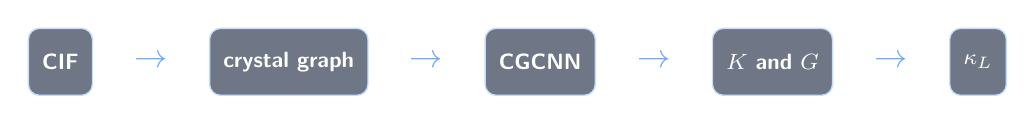
\begin{tikzpicture}[node distance=4mm,
  pill/.style={rounded corners=4pt, fill=Navy!60, draw=LightBlue!40,
               line width=0.5pt, minimum height=0.85cm, align=center,
               inner sep=5pt, font=\sffamily\bfseries\footnotesize\color{white}},
  arr/.style={font=\color{LightBlue}\large}]
  \node[pill] (n1) {CIF};
  \node[arr, right=of n1] (a1) {$\rightarrow$};
  \node[pill, right=of a1] (n2) {crystal graph};
  \node[arr, right=of n2] (a2) {$\rightarrow$};
  \node[pill, right=of a2] (n3) {CGCNN};
  \node[arr, right=of n3] (a3) {$\rightarrow$};
  \node[pill, right=of a3] (n4) {$K$ and $G$};
  \node[arr, right=of n4] (a4) {$\rightarrow$};
  \node[pill, right=of a4] (n5) {$\kappa_L$};
\end{tikzpicture}\\[16pt]
{\color{Subtle}\sffamily\small Aizaz Khalid \quad$\cdot$\quad
  reproduction of PINK, J.\ Mater.\ Inf.\ 2025, 5, 12}
\end{center}
\end{frame}
\endgroup

% =============================================================================
% PART 1 - MOTIVATION
% =============================================================================

\begin{frame}
\SlideHeader{01 \textperiodcentered\ MOTIVATION}{Why predict elastic moduli at all?}

\begin{columns}[T]
\column{0.485\linewidth}
\Card{4.55cm}{CardBg}{CardRule}{%
  {\headingfont\bfseries\large\color{SlideInk} The bottleneck}\\[4pt]
  \sffamily\small
  Elastic moduli come from DFT calculations costing hours to days of
  compute --- only $\sim$11{,}000 of the Materials Project's
  $\sim$150{,}000 entries have them.\\[4pt]
  Screening a large candidate space by DFT alone is not affordable.}

\column{0.485\linewidth}
\Card{4.55cm}{CardBg}{CardRule}{%
  {\headingfont\bfseries\large\color{SlideInk} Why they matter here}\\[4pt]
  \sffamily\small
  PINK screens for materials with ultralow \emph{lattice thermal
  conductivity} $\kappa_L$, whose physics stage needs bulk modulus $K$ and
  shear modulus $G$ as inputs.\\[4pt]
  Predicting $K$ and $G$ in milliseconds turns an impossible screen into a
  routine one.}
\end{columns}

\Takeaway{A CIF file says where the atoms are. It does not say how stiff the
crystal is --- that is what we are learning to predict.}
\end{frame}

% -----------------------------------------------------------------------------
\begin{frame}
\SlideHeader{02 \textperiodcentered\ MOTIVATION}{Why not just a standard neural network?}

\sffamily\footnotesize
A dense network expects a fixed-length vector; a CNN expects a fixed-size
grid. Neither fits a crystal:

\vspace{3pt}
\begin{columns}[T]
\column{0.32\linewidth}
\Card{3.9cm}{CardBg}{CardRule}{%
  {\bfseries\footnotesize\color{SlideInk} Variable size}\\[3pt]
  \footnotesize A unit cell can hold 2 atoms or 200 --- no fixed vector
  length to build a dense layer around.}
\column{0.32\linewidth}
\Card{3.9cm}{CardBg}{CardRule}{%
  {\bfseries\footnotesize\color{SlideInk} No grid}\\[3pt]
  \footnotesize Atoms sit at arbitrary 3D positions, not on the regular
  pixel grid a CNN's kernel slides across.}
\column{0.32\linewidth}
\Card{3.9cm}{CardBg}{CardRule}{%
  {\bfseries\footnotesize\color{SlideInk} It repeats forever}\\[3pt]
  \footnotesize A crystal is periodic --- tiling space in three directions,
  not croppable to a fixed patch.}
\end{columns}

\vspace{4pt}
\Card{11.7cm}{BlueBg}{SlideBlue}{%
  \sffamily\footnotesize\color{SlideInk}
  \textbf{The fix: represent it as a \emph{graph}} --- atoms as nodes,
  bonds as edges --- which natively handles a variable number of objects in
  arbitrary positions. A graph neural network passes messages along the
  edges instead of convolving over pixels; CGCNN is exactly this, built for
  crystals.}

\Takeaway{Everything from here on is about the two things a graph needs:
a node, and an edge.}
\end{frame}

% -----------------------------------------------------------------------------
\begin{frame}
\SlideHeader{03 \textperiodcentered\ THE PIPELINE}{Where this project fits inside PINK}

\begin{center}
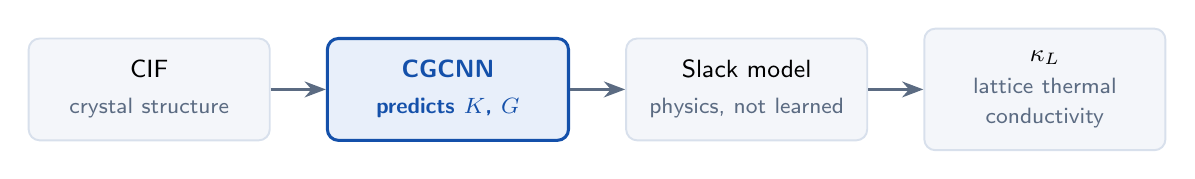
\begin{tikzpicture}[node distance=7mm,
  box/.style={rounded corners=4pt, draw=CardRule, fill=CardBg, line width=0.7pt,
              text width=2.5cm, align=center, inner sep=8pt, font=\sffamily\small},
  hl/.style={rounded corners=4pt, draw=SlideBlue, fill=BlueBg, line width=1.1pt,
             text width=2.5cm, align=center, inner sep=8pt,
             font=\sffamily\bfseries\small\color{SlideBlue}},
  arr/.style={-{Stealth[length=2.7mm]}, line width=0.9pt, draw=Muted}]
  \node[box] (cif) {CIF\\[2pt]\footnotesize\color{Muted} crystal structure};
  \node[hl, right=of cif] (cgcnn) {CGCNN\\[2pt]\footnotesize predicts $K$, $G$};
  \node[box, right=of cgcnn] (slack) {Slack model\\[2pt]\footnotesize\color{Muted} physics, not learned};
  \node[box, right=of slack] (kl) {$\kappa_L$\\[2pt]\footnotesize\color{Muted} lattice thermal\\ conductivity};
  \draw[arr] (cif) -- (cgcnn);
  \draw[arr] (cgcnn) -- (slack);
  \draw[arr] (slack) -- (kl);
\end{tikzpicture}
\end{center}

\vspace{5pt}
{\sffamily\large\bfseries\color{SlideInk}
The elastic moduli are the \emph{only} learned quantity. Everything
downstream of them is physics, not machine learning.}

\vspace{4pt}
{\sffamily\small\color{Muted}
This project implements the first arrow --- CIF $\rightarrow$ $(K,G)$ ---
including the network itself, written from scratch rather than forked from
the paper's code. Its output is the $(K,G)$ table the $\kappa_L$ stage
consumes.}

\Takeaway{Scope of this talk: the machine-learning half of PINK, explained
from first principles and reproduced independently.}
\end{frame}

% =============================================================================
\begin{dividerframe}
\begin{center}
{\color{LightBlue}\bfseries\sffamily\large PART TWO}\\[8pt]
{\color{white}\bfseries\headingfont\fontsize{30}{36}\selectfont
  From Crystal to Graph}\\[9pt]
{\color{Subtle}\sffamily\normalsize
  Nodes, edges, and a worked example in real sodium chloride}
\end{center}
\end{dividerframe}

% -----------------------------------------------------------------------------
\begin{frame}
\SlideHeader{04 \textperiodcentered\ CRYSTAL TO GRAPH}{Meet the crystal: rock-salt NaCl}

\begin{columns}[T]
\column{0.52\linewidth}
{\sffamily\footnotesize
Ordinary table salt. Its structure --- \textbf{rock salt} --- is one of the
simplest in nature, and every number here comes from the actual CIF file
used throughout this talk.}

\vspace{3pt}
\Card{6.0cm}{CardBg}{CardRule}{%
  \sffamily\footnotesize
  \textbf{Cubic cell, side $a = 5.62$ \AA}\\[2pt]
  8 ions per cell: 4 Na$^+$, 4 Cl$^-$.\\[2pt]
  Every Na$^+$ sits surrounded by 6 Cl$^-$ neighbours, all at exactly
  $a/2 = 2.81$ \AA\ --- the real crystal's coordination, not a
  simplification.}

\column{0.44\linewidth}
{\sffamily\footnotesize\color{Muted} Fractional coordinates, from the CIF:}\\[2pt]
\begin{tabular}{@{}lccc@{}}
\toprule
\footnotesize ion & \footnotesize $x$ & \footnotesize $y$ & \footnotesize $z$ \\
\midrule
\footnotesize Na$^+$ & 0 & 0 & 0 \\
\footnotesize Na$^+$ & 0 & 0.5 & 0.5 \\
\footnotesize Na$^+$ & 0.5 & 0 & 0.5 \\
\footnotesize Na$^+$ & 0.5 & 0.5 & 0 \\
\footnotesize Cl$^-$ & 0.5 & 0.5 & 0.5 \\
\footnotesize Cl$^-$ & 0.5 & 0 & 0 \\
\footnotesize Cl$^-$ & 0 & 0.5 & 0 \\
\footnotesize Cl$^-$ & 0 & 0 & 0.5 \\
\bottomrule
\end{tabular}
\end{columns}

\Takeaway{A CIF is nothing more than a table like this one, plus the cell
size and shape. Turning it into a graph is the next three slides.}
\end{frame}

% -----------------------------------------------------------------------------
\begin{frame}
\SlideHeader{05 \textperiodcentered\ CRYSTAL TO GRAPH}{Nodes, edges, and a cutoff radius}

\begin{columns}[T]
\column{0.60\linewidth}
\includegraphics[height=4.6cm]{nacl_crystal}

\column{0.37\linewidth}
{\sffamily\footnotesize
\textbf{\color{SlideBlue}Nodes = atoms.} Every ion in the faded, infinite
lattice is one node.\\[3pt]
\textbf{\color{SlideBlue}Edges = bonds} to neighbours \emph{within a cutoff
radius $r$} only (bold, $r\approx2.9$ \AA\ here).\\[3pt]
For this Cl$^-$, that cutoff catches exactly its 6 nearest Na$^+$.}
\end{columns}

\Takeaway{In the real pipeline, $r=8$ \AA\ and up to 12 neighbours are kept
per atom --- the idea is identical, just with more neighbours in view.}
\end{frame}

% -----------------------------------------------------------------------------
\begin{frame}
\SlideHeader{06 \textperiodcentered\ CRYSTAL TO GRAPH}{The abstraction: what the network sees}

\begin{columns}[T]
\column{0.56\linewidth}
\includegraphics[height=4.6cm]{nacl_graph}

\column{0.40\linewidth}
{\sffamily\small
Strip away the projection, the perspective, the rest of the crystal fading
into the background --- and this is what is left: one small, labelled
graph.\\[6pt]
No 3D coordinates are given to the network directly. Only:}
\vspace{3pt}
\begin{itemize}
\setlength\itemsep{5pt}
\small
\item which atom each node is
\item which pairs of atoms are connected
\item how far apart each connected pair is
\end{itemize}
\end{columns}

\Takeaway{This is not a simplification of what CGCNN sees --- it \emph{is}
what CGCNN sees. A crystal, to this network, is exactly this object.}
\end{frame}

% -----------------------------------------------------------------------------
\begin{frame}
\SlideHeader{07 \textperiodcentered\ CRYSTAL TO GRAPH}{What's inside a node}

{\sffamily\footnotesize
Each node must carry \emph{what element it is}. Rather than learning this
from scratch, every atom is looked up in a fixed table.}

\vspace{4pt}
\begin{columns}[T]
\column{0.60\linewidth}
\Card{7.2cm}{CardBg}{CardRule}{%
  \sffamily\footnotesize
  \textbf{\texttt{atom\_init.json}}: one 92-dimensional vector per element,
  built once from tabulated properties --- group, period,
  electronegativity, covalent radius, valence count --- one-hot
  binned.\\[3pt]
  These numbers are \textbf{fixed, never learned} --- the starting
  description of ``what element is this'', identical for every atom of a
  given element in the dataset.}

\column{0.36\linewidth}
\Card{4.3cm}{BlueBg}{SlideBlue}{%
  \sffamily\footnotesize\color{SlideInk}
  \textbf{The network's first layer} is a linear projection turning this
  fixed 92-dim description into the model's hidden width --- the one place
  element identity becomes something \emph{learned}.}
\end{columns}

\Takeaway{Analogous to a lookup embedding table in NLP --- except these
starting vectors are physically meaningful, not randomly initialised.}
\end{frame}

% -----------------------------------------------------------------------------
\begin{frame}
\SlideHeader{08 \textperiodcentered\ CRYSTAL TO GRAPH}{Expanding the bond length}

{\sffamily\footnotesize A bond has one obvious number: its length. Feeding
that number in raw turns out to be a bad idea.}

\vspace{3pt}
\Card{11.9cm}{CardBg}{CardRule}{%
  \centering\headingfont\bfseries\fontsize{12.5}{15}\selectfont\color{SlideInk}
  $e_k(d) \!=\! \exp\!\left(-\dfrac{(d-\mu_k)^2}{\sigma^2}\right)
  \;\; \mu_k \!=\! 0,0.2,\dots,8\text{ \AA} \;\; \sigma \!=\! 0.2\text{ \AA}$}

\vspace{4pt}
\begin{columns}[T]
\column{0.485\linewidth}
\Card{5.5cm}{CardBg}{CardRule}{%
  {\footnotesize\bfseries\color{SlideInk} The problem with one number}\\[2pt]
  \sffamily\footnotesize
  A single scalar forces the network to learn a sharply non-linear
  response from scratch --- hard to fit, slow to converge.}
\column{0.485\linewidth}
\Card{5.5cm}{CardBg}{CardRule}{%
  {\footnotesize\bfseries\color{SlideInk} What the expansion buys}\\[2pt]
  \sffamily\footnotesize
  A 2.31 \AA\ bond lights up the basis functions near 2.3, barely touching
  the one at 5.0 --- smooth and easy to learn, not a cliff.}
\end{columns}

\Takeaway{This is a radial basis expansion --- the same trick used
throughout atomistic machine learning, not something specific to CGCNN.}
\end{frame}

% -----------------------------------------------------------------------------
\begin{frame}
\SlideHeader{09 \textperiodcentered\ CRYSTAL TO GRAPH}{Assembling one training example}

{\sffamily\small For a crystal of $N$ atoms, the graph handed to the
network is exactly three tensors:}

\vspace{3pt}
\begin{columns}[T]
\column{0.32\linewidth}
\Card{3.85cm}{GreenBg}{GreenRule}{%
  \sffamily\small
  \textbf{\color{SlideGreen}Atom features}\\[2pt]
  $N \times 92$\\[2pt]
  one fixed row per atom}
\column{0.32\linewidth}
\Card{3.85cm}{BlueBg}{SlideBlue}{%
  \sffamily\small
  \textbf{\color{SlideBlue}Bond features}\\[2pt]
  $N \times 12 \times 41$\\[2pt]
  Gaussian-expanded distance to each of up to 12 neighbours}
\column{0.32\linewidth}
\Card{3.85cm}{AmberBg}{AmberRule}{%
  \sffamily\small
  \textbf{\color{SlideAmber}Neighbour index}\\[2pt]
  $N \times 12$\\[2pt]
  which row of the atom table each neighbour is}
\end{columns}

\vspace{6pt}
{\sffamily\small\color{Muted}
This triple, plus the true modulus in GPa, is one row of training data. The
periodic neighbour search that builds it is the single slowest step in the
whole pipeline --- for 10{,}987 crystals it is computed once and cached.}

\Takeaway{Every crystal in this project, no matter how large or exotic, is
reduced to exactly this shape before it ever reaches the network.}
\end{frame}

% =============================================================================
\begin{dividerframe}
\begin{center}
{\color{LightBlue}\bfseries\sffamily\large PART THREE}\\[8pt]
{\color{white}\bfseries\headingfont\fontsize{30}{36}\selectfont
  The Network Itself}\\[9pt]
{\color{Subtle}\sffamily\normalsize
  How the graph turns into one number}
\end{center}
\end{dividerframe}

% -----------------------------------------------------------------------------
\begin{frame}
\SlideHeader{10 \textperiodcentered\ THE NETWORK}{In plain words, before the equations}

\vspace{3pt}
\Card{11.9cm}{BlueBg}{SlideBlue}{%
  \sffamily\large\color{SlideInk}
  \textit{``Each atom asks its neighbours: what are you, and how far away?
  Then it updates its own description based on the answers it hears.''}}

\vspace{8pt}
{\sffamily\small
That single round of asking-and-updating is called \textbf{message
passing}, and it is the entire idea behind the network's convolution step.
Do it once, and every atom's description reflects its immediate neighbours.
Do it three times --- as this network does --- and every atom's
description reflects everything happening within three bonds of it.}

\vspace{5pt}
{\sffamily\small\color{Muted}
The next slide formalises exactly this sentence as an equation. Nothing
new is being introduced --- only made precise.}

\Takeaway{If the equations on the next slide feel abstract, come back to
this sentence. That is all they are computing.}
\end{frame}

% -----------------------------------------------------------------------------
\begin{frame}
\SlideHeader{11 \textperiodcentered\ THE NETWORK}{The gated convolution}

{\sffamily\small For atom $i$ with neighbours $j$, form the (self,
neighbour, bond) triple for every edge, then update:}

\vspace{4pt}
\Card{11.9cm}{CardBg}{CardRule}{%
\centering
$z_{ij} = v_i \oplus v_j \oplus e_{ij}$\\[6pt]
{\headingfont\bfseries\fontsize{16}{20}\selectfont\color{SlideBlue}
$v_i \;\leftarrow\; v_i \;+\; \displaystyle\sum_{j}
   \sigma(z_{ij}W_f + b_f) \;\odot\; g(z_{ij}W_s + b_s)$}}

\vspace{5pt}
{\sffamily\footnotesize\color{Muted}
$\oplus$ concatenation $\quad\odot$ elementwise product $\quad\sigma$
sigmoid (the gate) $\quad g$ softplus (the message) $\quad v_i$ the running
description of atom $i$}

\vspace{5pt}
{\sffamily\small
One shared linear layer processes every edge in the entire crystal
identically. That sharing is what makes this a \emph{convolution}: the same
local rule applies everywhere, whether the crystal has 8 atoms or 200.}

\Takeaway{This one update, stacked three times, is the entire learned part
of turning a graph into a description of the crystal.}
\end{frame}

% -----------------------------------------------------------------------------
\begin{frame}
\SlideHeader{12 \textperiodcentered\ THE NETWORK}{Three design choices, and why}

\begin{columns}[T]
\column{0.32\linewidth}
\AccentCard{3.85cm}{SlideBlue}{%
  \sffamily\small
  {\bfseries\color{SlideBlue}The gate $\sigma(\cdot)$}\\[3pt]
  Decides, per bond, how much that neighbour contributes. A weak, distant
  bond can be down-weighted without being deleted from the graph.}
\column{0.32\linewidth}
\AccentCard{3.85cm}{SlideGreen}{%
  \sffamily\small
  {\bfseries\color{SlideGreen}Shared weights}\\[3pt]
  The same linear layer processes every edge. That is what makes this a
  convolution, and why it generalises across crystal sizes.}
\column{0.32\linewidth}
\AccentCard{3.85cm}{SlideAmber}{%
  \sffamily\small
  {\bfseries\color{SlideAmber}The residual, $v_i + (\cdot)$}\\[3pt]
  Gradients flow straight through the stack, so early layers are not washed
  out by later ones as three layers compound.}
\end{columns}

\Takeaway{Three convolution layers are used here, so every atom's final
description reflects roughly a three-bond-hop neighbourhood.}
\end{frame}

% -----------------------------------------------------------------------------
\begin{frame}
\SlideHeader{13 \textperiodcentered\ THE NETWORK}{Stacking layers grows the neighbourhood}

\begin{center}
\scalebox{0.62}{
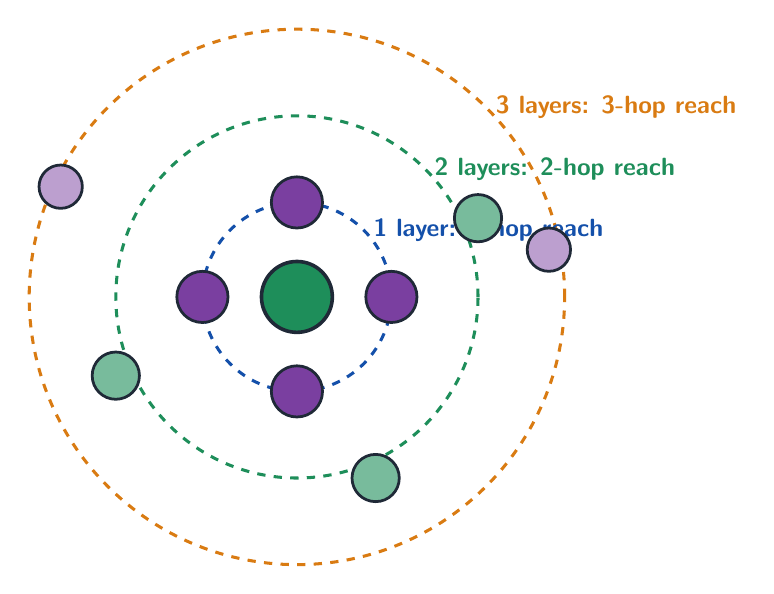
\begin{tikzpicture}
  \foreach \r/\lab/\c in {3.4/{3 layers: 3-hop reach}/SlideAmber,
                           2.3/{2 layers: 2-hop reach}/SlideGreen,
                           1.2/{1 layer: 1-hop reach}/SlideBlue} {
    \draw[\c, dashed, line width=1.1pt] (0,0) circle (\r);
    \node[font=\sffamily\bfseries\small, color=\c, anchor=west]
      at ({45}:{\r}) {\lab};
  }
  \node[circle, fill=ClColor, draw=SlideInk, line width=1.3pt, minimum size=9mm]
       at (0,0) {};
  \node[circle, fill=NaColor, draw=SlideInk, line width=1pt, minimum size=6.5mm] at (1.2,0) {};
  \node[circle, fill=NaColor, draw=SlideInk, line width=1pt, minimum size=6.5mm] at (-1.2,0) {};
  \node[circle, fill=NaColor, draw=SlideInk, line width=1pt, minimum size=6.5mm] at (0,1.2) {};
  \node[circle, fill=NaColor, draw=SlideInk, line width=1pt, minimum size=6.5mm] at (0,-1.2) {};
  \node[circle, fill=ClColor!60, draw=SlideInk, line width=1pt, minimum size=6mm] at (2.3,1.0) {};
  \node[circle, fill=ClColor!60, draw=SlideInk, line width=1pt, minimum size=6mm] at (-2.3,-1.0) {};
  \node[circle, fill=ClColor!60, draw=SlideInk, line width=1pt, minimum size=6mm] at (1.0,-2.3) {};
  \node[circle, fill=NaColor!50, draw=SlideInk, line width=1pt, minimum size=5.5mm] at (3.2,0.6) {};
  \node[circle, fill=NaColor!50, draw=SlideInk, line width=1pt, minimum size=5.5mm] at (-3.0,1.4) {};
\end{tikzpicture}}
\end{center}

{\sffamily\footnotesize\centering
Each additional layer lets information travel one more bond hop. After 3
layers, the centre atom's description is shaped by every atom within 3
bonds --- with no global, whole-crystal operation ever computed.}

\Takeaway{More layers see further, at the cost of more computation and a
risk of over-smoothing --- which is why 3 is a deliberate choice, not a
default.}
\end{frame}

% -----------------------------------------------------------------------------
\begin{frame}
\SlideHeader{14 \textperiodcentered\ THE NETWORK}{From atoms to one number: pooling}

\begin{columns}[T]
\column{0.56\linewidth}
\Card{6.7cm}{GreenBg}{GreenRule}{%
  \centering{\headingfont\bfseries\fontsize{17}{20}\selectfont\color{SlideGreen}
  $v_c = \dfrac{1}{N}\displaystyle\sum_{i=1}^{N} v_i$}\\[6pt]
  \sffamily\small\raggedright\color{SlideInk}
  Average, not sum, over every atom's final vector to get one description
  of the whole crystal.}

\column{0.40\linewidth}
{\sffamily\small
A modulus is an \textbf{intensive} property --- doubling the unit cell must
not double the prediction.\\[4pt]
A \emph{sum} would make the output scale with however many atoms the CIF
author happened to write down. The \emph{mean} does not.}
\end{columns}

\vspace{5pt}
{\sffamily\small\color{Muted}
A small fully-connected head then turns that one 128-dimensional vector
into a single number: the predicted modulus.}

\Takeaway{This is the one place the model has to actively resist a bias
the data would otherwise hand it for free.}
\end{frame}

% -----------------------------------------------------------------------------
\begin{frame}
\SlideHeader{15 \textperiodcentered\ THE NETWORK}{What we predict, and why its logarithm}

\begin{columns}[T]
\column{0.485\linewidth}
\Card{5.35cm}{AmberBg}{AmberRule}{%
  {\bfseries\color{SlideAmber} Train on $\log_{10}(\text{modulus})$}\\[3pt]
  \sffamily\small
  Moduli here span 1--575 GPa. Under plain MSE on raw values, a 40 GPa
  error on a stiff crystal produces $100\times$ more gradient than the same
  \emph{relative} error on a soft one.}

\column{0.485\linewidth}
\Card{5.35cm}{RedBg}{RedRule}{%
  {\bfseries\color{SlideRed} Exactly the wrong bias here}\\[3pt]
  \sffamily\small
  PINK screens for \textbf{ultralow} conductivity --- the soft end of the
  range. A model that only cares about stiff crystals is worthless for
  this project's actual goal.}
\end{columns}

\vspace{5pt}
{\sffamily\small
The logarithm converts ``within a factor of $x$'' into ``within a fixed
distance'' --- so soft and stiff crystals carry equal weight during
training. Normalisation statistics (mean, std) come from the training
split only, so no information about held-out crystals leaks in.}

\Takeaway{This single transform is why the model is not simply best at
predicting hard, boring materials.}
\end{frame}

% -----------------------------------------------------------------------------
\begin{frame}
\SlideHeader{16 \textperiodcentered\ THE NETWORK}{The full forward pass, start to finish}

\begin{center}
\resizebox{\linewidth}{!}{%
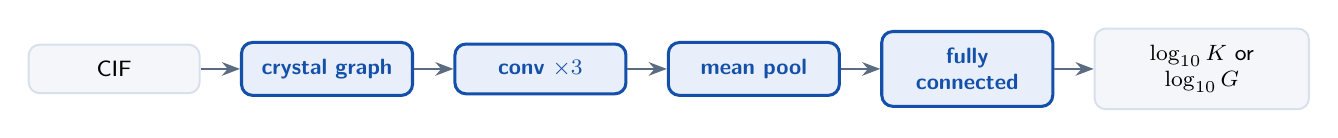
\begin{tikzpicture}[node distance=5mm,
  box/.style={rounded corners=4pt, draw=CardRule, fill=CardBg, line width=0.7pt,
              text width=1.75cm, align=center, inner sep=6pt, font=\sffamily\footnotesize},
  hl/.style={rounded corners=4pt, draw=SlideBlue, fill=BlueBg, line width=1.1pt,
             text width=1.75cm, align=center, inner sep=6pt,
             font=\sffamily\bfseries\footnotesize\color{SlideBlue}},
  arr/.style={-{Stealth[length=2.3mm]}, line width=0.8pt, draw=Muted}]
  \node[box] (a) {CIF};
  \node[hl, right=of a] (b) {crystal graph};
  \node[hl, right=of b] (c) {conv $\times 3$};
  \node[hl, right=of c] (d) {mean pool};
  \node[hl, right=of d] (e) {fully\\connected};
  \node[box, right=of e, text width=2.3cm] (f) {$\log_{10} K$ or $\log_{10} G$};
  \draw[arr] (a)--(b); \draw[arr] (b)--(c); \draw[arr] (c)--(d);
  \draw[arr] (d)--(e); \draw[arr] (e)--(f);
\end{tikzpicture}}
\end{center}

\vspace{7pt}
{\sffamily\small\centering
Every piece of this diagram has now been explained: how a crystal becomes a
graph (Part 2), what the convolution and pooling steps do and why (this
part), and why the target is a logarithm. Nothing else is hidden inside
this network.}

\Takeaway{80{,}833 parameters in total --- small by deep-learning standards,
because the graph representation already does most of the work.}
\end{frame}

% =============================================================================
\begin{dividerframe}
\begin{center}
{\color{LightBlue}\bfseries\sffamily\large PART FOUR}\\[8pt]
{\color{white}\bfseries\headingfont\fontsize{30}{36}\selectfont
  Our Data and Training}\\[9pt]
{\color{Subtle}\sffamily\normalsize
  What to train on, and how three models beat one}
\end{center}
\end{dividerframe}

% -----------------------------------------------------------------------------
\begin{frame}
\SlideHeader{17 \textperiodcentered\ OUR DATA}{What to train on}

\begin{columns}[T]
\column{0.485\linewidth}
\Card{4.3cm}{CardBg}{CardRule}{%
  \sffamily\footnotesize
  \textbf{1{,}213 CIFs} --- Materials Project structures, no labels. The
  \textbf{prediction} set.}
\column{0.485\linewidth}
\Card{4.3cm}{BlueBg}{SlideBlue}{%
  \sffamily\footnotesize\color{SlideInk}
  \textbf{10{,}987 matbench crystals} --- DFT-computed $K,G$, the paper's
  own benchmark. The \textbf{training} set.}
\end{columns}

\vspace{3pt}
{\sffamily\footnotesize
Only 278 of the 1{,}213 appear in matbench --- tempting to label just those.}

\vspace{3pt}
\Card{11.9cm}{AmberBg}{AmberRule}{%
  {\footnotesize\bfseries\color{SlideAmber} The structures were never the
  limit --- the labels were}\\[2pt]
  \sffamily\footnotesize\color{SlideInk}
  Intersecting an unlabelled collection with a labelled benchmark discards
  97\% of the labels that exist. Invert the roles: train on all 10{,}987
  matbench crystals, treat the 1{,}213 CIFs purely as a prediction
  set --- 40$\times$ more training data, and what the paper itself does.}

\Takeaway{When labels are the scarce resource, never let an unlabelled
collection define the training set.}
\end{frame}

% -----------------------------------------------------------------------------
\begin{frame}
\SlideHeader{18 \textperiodcentered\ OUR DATA}{Three models, averaged}

{\sffamily\small
Two networks trained on the same data with different random
initialisations land in different minima. They \textbf{agree} about the
signal and \textbf{disagree} about their own noise --- so averaging keeps
the first and partly cancels the second.}

\vspace{4pt}
\begin{columns}[T]
\column{0.32\linewidth}
\AccentCard{3.85cm}{SlideBlue}{%
  \sffamily\small{\bfseries\color{SlideBlue}Average in log space}\\[3pt]
  10 and 1000 GPa average to 100 GPa in log space, 505 GPa linearly. 100 is
  the defensible answer.}
\column{0.32\linewidth}
\AccentCard{3.85cm}{SlideGreen}{%
  \sffamily\small{\bfseries\color{SlideGreen}One shared split}\\[3pt]
  Initialisation varies between the three models; the train/val/test split
  does not --- or the ensemble's score is measured partly on data some
  member trained on.}
\column{0.32\linewidth}
\AccentCard{3.85cm}{SlideAmber}{%
  \sffamily\small{\bfseries\color{SlideAmber}Free uncertainty}\\[3pt]
  Spread between the three predictions is a per-crystal confidence signal
  --- large spread means the ensemble is guessing.}
\end{columns}

\Takeaway{Ensembling typically buys 10--15\% lower error. Ours gained
\EnsembleGainPct\%\ on bulk modulus, in that range.}
\end{frame}

% =============================================================================
\begin{dividerframe}
\begin{center}
{\color{LightBlue}\bfseries\sffamily\large PART FIVE}\\[8pt]
{\color{white}\bfseries\headingfont\fontsize{30}{36}\selectfont Results}\\[9pt]
{\color{Subtle}\sffamily\normalsize
  How well it actually works}
\end{center}
\end{dividerframe}

% -----------------------------------------------------------------------------
\begin{frame}
\SlideHeader{19 \textperiodcentered\ RESULTS}{Model performance}

\begin{center}
\small
\begin{tabular}{@{}lcccc@{}}
\toprule
\textbf{Model} & \textbf{MAE $\log_{10}$(GPa)} & \textbf{$R^2$} &
  \textbf{MAE (GPa)} & \textbf{Rel.\ error} \\
\midrule
Bulk, single model & \KOneMae & \KOneRtwo & \KOneGpa & \KOneRel\% \\
\textbf{$\blacktriangleright$ Bulk, 3-model ensemble} & \textbf{\KEnsMae} &
  \textbf{\KEnsRtwo} & \textbf{\KEnsGpa} & \textbf{\KEnsRel\%} \\
Shear, single model & \GOneMae & \GOneRtwo & \GOneGpa & \GOneRel\% \\
\textbf{$\blacktriangleright$ Shear, 3-model ensemble} & \textbf{\GEnsMae} &
  \textbf{\GEnsRtwo} & \textbf{\GEnsGpa} & \textbf{\GEnsRel\%} \\
\bottomrule
\end{tabular}
\end{center}

\vspace{3pt}
{\sffamily\footnotesize\color{Muted}\centering
Measured on 1{,}648 held-out crystals. All models share one
train/validation/test split, so every row is directly comparable.}

\vspace{5pt}
\begin{columns}[T]
\column{0.485\linewidth}
\Card{5.35cm}{GreenBg}{GreenRule}{%
  {\bfseries\color{SlideGreen}No overfitting}\\[3pt]
  \sffamily\small
  Train \KTrainMae\ vs.\ test \KEnsMae\ --- ordinary generalisation error,
  not recall.}
\column{0.485\linewidth}
\Card{5.35cm}{BlueBg}{SlideBlue}{%
  {\bfseries\color{SlideBlue}Ensembling gain}\\[3pt]
  \sffamily\small\color{SlideInk}
  \EnsembleGainPct\% of the bulk-modulus error removed by averaging three
  initialisations.}
\end{columns}
\end{frame}

% -----------------------------------------------------------------------------
\begin{frame}
\SlideHeader{20 \textperiodcentered\ RESULTS}{How we compare to the literature}

\begin{columns}[T]
\column{0.60\linewidth}
\includegraphics[width=\linewidth]{literature}
\column{0.36\linewidth}
{\sffamily\small
\textbf{Reading this:} our bulk ensemble slightly \textbf{beats} the paper
it reproduces.\\[4pt]
It sits between PINK and coGN --- the best result ever published on this
benchmark, with any architecture.\\[4pt]
Same architecture, same training data as the paper. The gain comes from
ensembling and a cosine learning-rate schedule.}
\end{columns}

\Takeaway{Reproduction target met: \KEnsMae\ against the paper's
$\approx$0.070.}
\end{frame}

% -----------------------------------------------------------------------------
\begin{frame}
\SlideHeader{21 \textperiodcentered\ RESULTS}{Predicted vs.\ DFT --- bulk modulus}

\begin{columns}[T]
\column{0.50\linewidth}

\includegraphics[height=5.4cm]{parity_K_VRH_ens}
\column{0.46\linewidth}
{\sffamily\small
Every point is one crystal: DFT value on $x$, our prediction on $y$. A
perfect model puts every point on the diagonal.\\[4pt]
Points above the line are over-predictions; below, under-predictions.\\[4pt]
The shaded band marks ``within a factor of 1.5'' --- a useful screening
tolerance, where ranking matters more than the exact value.\\[4pt]
Blue = the 1{,}648 held-out test crystals. Grey = training data, shown for
context.}
\end{columns}

\Takeaway{$R^2 = \KEnsRtwo$ --- the model explains \KEnsRtwo\ of the
variance in bulk modulus across the whole test set.}
\end{frame}

% -----------------------------------------------------------------------------
\begin{frame}
\SlideHeader{22 \textperiodcentered\ RESULTS}{Predicted vs.\ DFT --- shear modulus}

\begin{columns}[T]
\column{0.50\linewidth}

\includegraphics[height=5.4cm]{parity_G_VRH_ens}
\column{0.46\linewidth}
{\sffamily\small
MAE \GEnsMae\ against \KEnsMae\ for bulk --- consistently worse, for a
physical reason.\\[4pt]
Bulk modulus resists uniform compression, dominated by average bond
stiffness --- close to what a graph network reads off directly.\\[4pt]
Shear modulus resists \emph{shape change}, which depends on bond
\emph{directionality} and anisotropy the representation captures less
directly.\\[4pt]
The same ordering appears in the paper and across the matbench
leaderboard --- a property of the task, not of this implementation.}
\end{columns}
\end{frame}

% -----------------------------------------------------------------------------
\begin{frame}
\SlideHeader{23 \textperiodcentered\ RESULTS}{Where the errors live}

\begin{center}

\includegraphics[height=4.3cm]{residuals_K_VRH_ens}
\end{center}

\vspace{3pt}
\begin{columns}[T]
\column{0.485\linewidth}
{\sffamily\small\textbf{\color{SlideGreen}Left: unbiased.} The error
distribution centres on zero --- the model does not systematically over- or
under-predict.}
\column{0.485\linewidth}
{\sffamily\small\textbf{\color{SlideAmber}Right: the honest weakness.}
Errors fan out below $\sim$30 GPa --- least reliable on soft materials,
precisely the ultralow-$\kappa$ regime PINK targets.}
\end{columns}
\end{frame}

% -----------------------------------------------------------------------------
\begin{frame}
\SlideHeader{24 \textperiodcentered\ RESULTS}{Ensembling, and how it trains}

\begin{columns}[T]
\column{0.46\linewidth}
\includegraphics[height=3.6cm]{ensemble}\\[2pt]
{\sffamily\footnotesize\color{Muted}
Consistent gains on both targets --- about \EnsembleGainPct\% of the error,
in line with the 10--15\% typically expected.}
\column{0.50\linewidth}
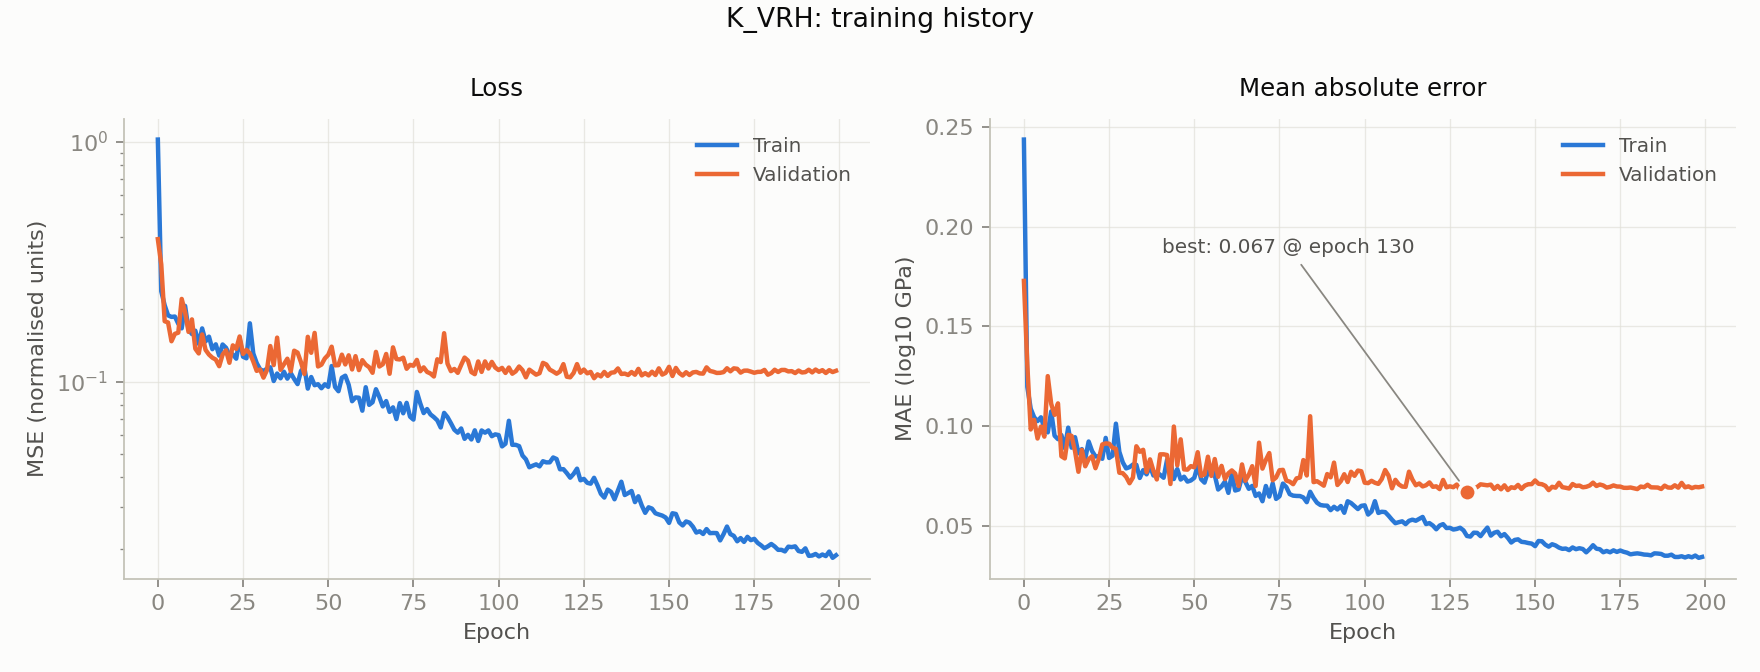
\includegraphics[height=3.6cm]{training_K_VRH_full}\\[2pt]
{\sffamily\footnotesize\color{Muted}
Cosine annealing over 200 epochs. Train and validation track closely
throughout --- no divergence, so no overfitting.}
\end{columns}
\end{frame}

% -----------------------------------------------------------------------------
\begin{frame}
\SlideHeader{25 \textperiodcentered\ RESULTS}{How low can the error go?}

{\sffamily\small
Because the model trains on $\log_{10}$, MAE converts to a
\textbf{multiplicative} error of $10^{\text{MAE}}-1$.}

\vspace{4pt}
\Card{11.9cm}{CardBg}{CardRule}{%
  \centering\headingfont\bfseries\fontsize{16}{19}\selectfont\color{SlideInk}
  MAE \KEnsMae\ $\rightarrow$ within a factor of \KFactor\ $\rightarrow$
  \KEnsRel\%\ typical error}

\vspace{5pt}
\Card{11.9cm}{RedBg}{RedRule}{%
  {\bfseries\color{SlideRed} A $\sim$2\% relative error is not reachable on
  this task --- by anyone}\\[3pt]
  \sffamily\small\color{SlideInk}
  2\% needs MAE $=0.0086$ --- about six times better than the best result
  ever published on this benchmark, with any architecture. The blocker is
  \textbf{label noise}, not model capacity: the targets are DFT-computed
  moduli, and DFT elastic constants themselves disagree with experiment by
  roughly 5--15\%. A model cannot be more accurate than the labels it is
  fitted to --- one reporting 2\% here would be revealing a leak, not an
  achievement.}

\Takeaway{Realistic floor for this architecture: $\approx$0.06 $\log_{10}$,
about 15\%. We are at \KEnsMae.}
\end{frame}

% =============================================================================
\begin{dividerframe}
\begin{center}
{\color{LightBlue}\bfseries\sffamily\large PART SIX}\\[8pt]
{\color{white}\bfseries\headingfont\fontsize{30}{36}\selectfont
  Wrapping Up}
\end{center}
\end{dividerframe}

% -----------------------------------------------------------------------------
\begin{frame}
\SlideHeader{26 \textperiodcentered\ CONTRIBUTION}{What we did differently from the paper}

\sffamily\footnotesize
\begin{enumerate}
\setlength\itemsep{4pt}
\item \textbf{Written from scratch} --- graph construction, convolution,
  pooling, training loop: our own implementation, not a fork. No
  pre-trained weights are ever loaded.
\item \textbf{Ensembles, not single models} --- three initialisations per
  target, averaged in log space, worth \EnsembleGainPct\% of the error and
  a per-crystal uncertainty the paper lacks.
\item \textbf{Adam with cosine annealing}, not the original's SGD with
  step decay --- a scheduled decay beats a reactive one on a fixed budget.
\item \textbf{Provenance on every prediction} --- each row records whether
  the model trained on that crystal, so recall is never mistaken for
  generalisation.
\item \textbf{A documented error floor} --- reporting both the
  multiplicative and range-normalised errors, not whichever flatters more.
\end{enumerate}

\Takeaway{Deliberately identical: the architecture, the training data, the
log target, the split ratio. In a reproduction, differences should be few
and intentional.}
\end{frame}

% -----------------------------------------------------------------------------
\begin{frame}
\SlideHeader{27 \textperiodcentered\ CONTRIBUTION}{The deliverable}

\Card{11.9cm}{BlueBg}{SlideBlue}{%
  {\headingfont\bfseries\large\color{SlideBlue}
  results/pink\_moduli\_predictions.csv}\\[4pt]
  \sffamily\small\color{SlideInk}
  Bulk and shear modulus for all 1{,}213 crystals --- with Pugh ratio, DFT
  reference where one exists, per-crystal ensemble uncertainty, and a
  provenance tag. This is the input the $\kappa_L$ stage consumes.}

\vspace{5pt}
\begin{columns}[T]
\column{0.32\linewidth}
\Card{3.4cm}{GreenBg}{GreenRule}{%
  \centering{\headingfont\bfseries\fontsize{22}{26}\selectfont\color{SlideGreen}935}\\[2pt]
  \sffamily\small\color{SlideInk} crystals genuinely unseen}
\column{0.32\linewidth}
\Card{3.4cm}{AmberBg}{AmberRule}{%
  \centering{\headingfont\bfseries\fontsize{22}{26}\selectfont\color{SlideAmber}278}\\[2pt]
  \sffamily\small\color{SlideInk} in matbench, tagged as recall}
\column{0.32\linewidth}
\Card{3.4cm}{BlueBg}{SlideBlue}{%
  \centering{\headingfont\bfseries\fontsize{22}{26}\selectfont\color{SlideBlue}42}\\[2pt]
  \sffamily\small\color{SlideInk} in the held-out test split}
\end{columns}

\Takeaway{A built-in correctness check: on those 42 test-provenance
crystals the error matches the benchmark test error exactly --- the
provenance mapping is doing its job.}
\end{frame}

% -----------------------------------------------------------------------------
\begin{frame}
\SlideHeader{28 \textperiodcentered\ CLOSING}{Summary}

\sffamily\small
\begin{itemize}
\setlength\itemsep{8pt}
\item A crystal is a \textbf{graph}: atoms as nodes, bonds within a cutoff
  as edges --- shown concretely in real NaCl.
\item A \textbf{gated convolution} lets each atom update its description
  from its neighbours; stacked three times, information travels three
  bonds.
\item \textbf{Mean pooling} and a \textbf{log-scale target} are both
  deliberate choices, not defaults --- one respects an intensive property,
  the other prevents the model from ignoring soft materials.
\item The scarce resource was \textbf{labels, not structures} --- training
  on all 10{,}987 matbench crystals rather than the 278-crystal overlap
  more than halved our error.
\item \textbf{Ensembling} three models bought a further \EnsembleGainPct\%,
  landing at \KEnsMae\ $\log_{10}$(GPa) for bulk modulus ---
  matching, and slightly beating, the paper this work reproduces.
\end{itemize}

\vspace{7pt}
\begin{center}
{\headingfont\bfseries\Large\color{SlideInk} Thank you.}
\end{center}
\end{frame}

\end{document}
